\documentclass[11pt,a4paper]{article}
\usepackage[T1]{fontenc}
\usepackage{graphicx}
\usepackage{array}
\usepackage{tabularx}
\usepackage[latin1]{inputenc}
\usepackage{mathtools}
\setlength{\topmargin}{-.5in}
\setlength{\textheight}{9in}
\setlength{\oddsidemargin}{.125in}
\setlength{\textwidth}{6.25in}
\begin{document}
\title{Parallel Algorithms Coursework}
\author{C\'edric DESSEZ, Valentin GRAND, Yann NICOLAS, Cyril NOVEL, Nicolas SERVEL}
\maketitle
\tableofcontents

\newpage

\section{Gathering the clues}
The first thing we did was to analyze in depth the evidence given by our intel. Hopefully the engineers from Nukehavistan were kind enough to leave clues about the computer system.

The very first thing we did was to find the identity of the man portrayed on the system. We were able to process the face into the database of Interpol, hoping we will find a rogue scientist working for the Nukehavistan. Unfortunately no match were found. We then used the ReverseImages tool Q made for us and found that the man was \textit{Leonhard Euler}, portrayed on a 1957 stamp of the USSR. Such a link supposes that the Nukehavistan is a communist nation and so a major threat to the democracy all around the world.

Because of the link with the USSR, we assumed that the funny writing above the clock was in Cyrillic script. As no one in our team was able to understand russian, we contacted the Translation Service of the MI-6. The translation was \textit{fast inverter integrated functions}.

The text below the clock is in french. As we are french, we perfectly understood it and it means \textit{Made in France}. However, it is very unlikely this machine was produced in France. The final design is ugly and everyone knows French are all about beauty and class. We assumed this was only a trick to harden our research.

\begin{figure}[!h]
\centering

\includegraphics[width=5cm]{oss.png}
\caption{The model of the classy French spy}
\label{frenchspy}
\end{figure}

We then took a look to the two sets of coordinates. The set along the board points to the lovely village of \textit{Beaumont-en-Auge} in France. Among the famous people born in this town, one stands out. \textit{Pierre Simon de Laplace} was a mathematician and his work could have highly interested the Nukehavistan. The second coordinates confirmed our idea : it points near the \textit{Laplace} RER station in Paris. We don't believe in coincidence. Laplace's work is the key of the system. The power to the minus one on the second set of coordinates strengthens our assumption about the \textit{inverter}.

We finally called the technical hotline. Since it is a charged number, we joined the bill at the end of the report. The technical hotline is only an answerbot. We tested if it was telling the truth by asking it the answer to the Ultimate Question of Life, the Universe and Everything. Since it answered 42, we assumed the bot was powerful enough to answer our upcoming questions\footnote{This raises serious issues about the advanced level of Nukehavistan in the Computer Science field. Maybe we should apply for a PhD in their university.}. When we asked what was in the box, it said \textit{Numerical Inversion of Laplace Transforms of Probability Distributions}. A quick and efficient DuckDuckGo search -- we made sure we weren't tracked -- pointed us to a research paper from 1995, presenting an algorithm using the Euler method for inverting Laplace transforms.

The loop was almost complete. We knew what the algorithm was and what to code. The only thing we didn't know was what the program was actually doing. We tried to reverse engineer the \textit{mystery.o} file. We obtained some strange figures.

\begin{figure}[!h]
\centering
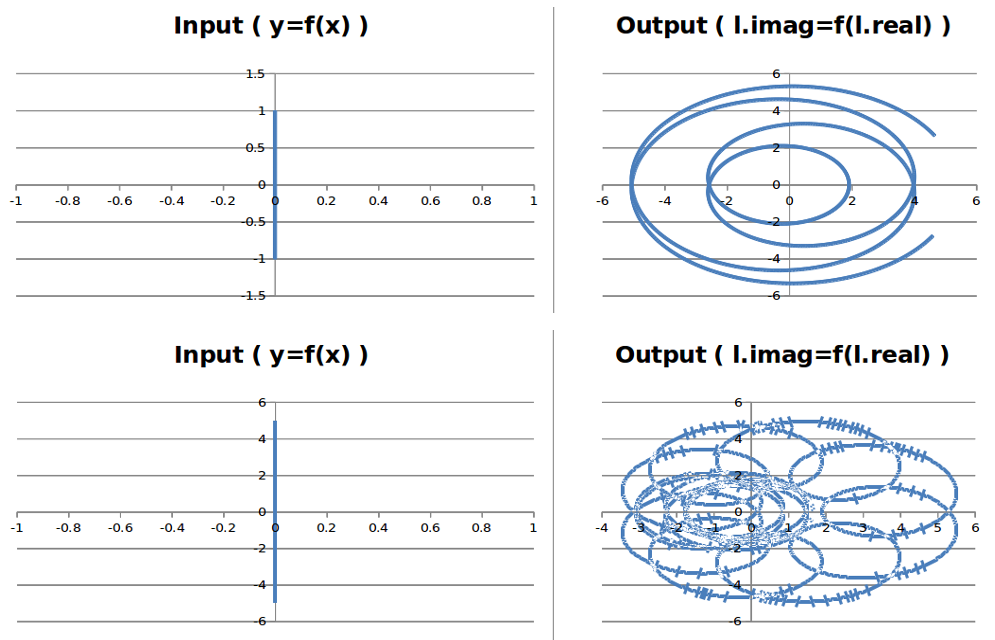
\includegraphics[width=10cm]{outputs.png}
\caption{Reverse engineering inputs and outputs.}
\label{reverse}
\end{figure}

We then made two assumptions. The first possibility is that the Nukehavistan is trying to communicate with superior life forces. The second possibility is that this computer system is prime in the job of the Nukehavistan spies. Since we are fierce scientists, we ruled out the first option. Thus we brainstormed over the second option by watching all the James Bond movies. At the end of this intensive marathon, we reached a conclusion :

\begin{figure}[!h]
\centering

\includegraphics[width=8cm]{watches.png}
\caption{Watches}
\label{reverse}
\end{figure}

Every spy needs a good watch! If we look closely to the computer system, the small peak of the output is on the 3 and the big peak is on the 11. The clock has its small hand pointing between 3 and 4 -- so in the 3 \textsuperscript{rd} hour. The large hand is pointing at 11. So the output of the computer system gives us the time!

\section{Implementation}

Since every good spy must be able to adapt and exploit their resources in the best possible way, they need a piece of software that is the fastest possible not only for an on-stage operation, but also when they are preparing the mission at the headquarters with access to the best super calculator in the world. This is why we have optimized this tremendous clock not only to run sequentially on a single machine, but also in parallel over several processes, multithreaded or not (depending on the given option), and distributed among a pool of machines.

\subsection{Sequential algorithm}

The first step in building this powerful clock is to implement and optimize the sequential algorithm. We first made a rough copy of the algorithm from the research paper and then modified it to make it more efficient and more flexible.\\

In the paper, the parameters \verb_N_ and \verb_M_ are hardcoded respectively to the values 15 and 11. That allows them to have a quite efficient processing and to hardcode the binomial coefficients. Those parameters determine the accuracy of the approximations done by the algorithm. After running a few tests, we realized that the more influent of those is \verb_N_ which we decided to set by default to $100$ (this also gives more computation to parallelize in the next steps). We have increased \verb_M_ a bit, up to $15$, to improve the accuracy, but also in anticipation of the parallelization which will use 16 machines.\\

In order to plot the inverted Laplace transform, we need to run this algorithm many times to obtain enough points. Thus we have strived to mutualise as much computation as possible. First the binomial coefficients are processed once and for all and saved to memory, as well as their sum which is in fact $2^M$ (hardcoded to $2048$ in the paper). Likewise, we process $exp(\frac{A}{2})$ only once for the whole set of points.\\

Besides, we have little interest here in the truncation error estimate, so we have got rid of the part of the code that processed it in the paper.\\

We have also merged the last two loops. As a matter of fact, filling an array \verb_SU_ with one loop to get \verb_Avgsu_ by summing its elements in a second loop is unefficient because we can do both at the same time which reduces the loop administration overhead and allows us to keep only a \verb_double_ variable instead of the array \verb_SU_.\\

We have also optimized the calculus of the variables \verb_i_ and \verb_Y_. In the paper they are computed with multiplications of float number, whereas there evolution corresponds to an incrementation by a fixed value at each iteration. Since in general an addition costs much less than a multiplication, this makes the loop faster. Notice there could be precision problems due to many successive foating point additions if \verb_M_ became much higher.\\

We are not sure whether or not those optimizations are substantial compared to the call to the mystery function, but it cannot do any harm anyways. Furthermore, since our class \verb_SeqLaplaceInv_ takes the function to invert as an argument, it might end up being useful to invert other functions less costly than our mystery function.

\subsection{Parallel MPI algorithm}

The program can be quite long when the size of the input increases. In order to accelerate what the machine does, we can use numerous processors in parallel. We call $N_p$ the number of processes. The program takes a vector of \verb_double_ as input, computes the algorithm for each data point and return a vector of \verb_double_ as output. We propose two different methods to parallelize the implementation:

\begin{itemize}

\item parallelizing the algorithm by rearranging the sequential algorithm,

\item dividing the input into chunks, and running in parallel the sequential algorithm on each chunk.

\end{itemize}

In both implementations, every process has to treat a certain amount of data. If we call $N_T$ the size of the total amount of data, each processor will treat a chunk of size $\lfloor \frac{N_T}{N_p} \rfloor$, and the "master" processor will treat the remaining $N_T-\lfloor \frac{N_T}{N_p} \rfloor$. It is not the most efficient way of handling the problem (even though in most cases the difference is negligible), but it is much easier to implement, because each processor except the master has the same amount of data to treat. 

\subsubsection{Parallel version of the algorithm}

In the sequential version of the algorithm, we have numerous sums. We want to calculate these sums in parallel but the problem is that each term of each sum depends on previous sums and one or more other terms. In order to parallelize the algorithm we have to come up with steps that are independent from each other.

\subsubsection*{Maths behind the parallelization}

The calculation of $Fun$ is the part of the algorithm we want to parallelize.

\begin{eqnarray}
	sum &=& \frac{1}{2}   \sum_{i=1}^{Ntr} (-1)^{i}fnRf(X,iH)\\
	SU(1) &=& sum  \\
	SU(k + 1) &=& SU(k) + (-1)^{Ntr+k}fnRf(X,(Ntr + k)H) \label{SU(i)}\\
	Fun &=&\frac{U}{Ctot} \sum_{i=1}^{M+1} \binom{M}{i-1}SU(i) \label{Fun}
\end{eqnarray}

We first notice that we can easily calculate $sum$ in parallel by calculating each term in parallel and then summing them. However, each $SU(i)$ needs $SU(i-1)$ to be calculated, so we must determine $Fun$ differently to design the algorithm.
We can rewrite \eqref{SU(i)} this way :
\begin{equation}
	SU(k) = sum + \sum_{i=1}^{k-1} (-1)^{Ntr+k-1}fnRf(X,(Ntr + k-1)H)
	\label{rewrite SU}
\end{equation}
In this case there are some values of $fnRf$ that are used by many $SU$, so that we lose time when we compute these expensive calculations more than once.
From \eqref{Fun} and \eqref{rewrite SU} we can rewrite a formulation for $Fun$ :
\begin{equation}
	Fun =\displaystyle{ \frac{U}{Ctot}  \sum_{k=1}^{M+1} \binom{M}{k-1}\left(sum + \sum_{i=1}^{k-1} (-1)^{Ntr+k-1}fnRf(X,(Ntr + k-1)H)\right)}
	\label{Fun2}
\end{equation}
We can change \eqref{Fun2} into :
\begin{eqnarray}
	S(1) &=& sum\\
	S(k) &=& (-1)^{Ntr+k-1}fnRf(X,(Ntr + k-1)H)\\
	Fun &=& \displaystyle{U \sum_{k=1}^{M+1}\left(S(k)(1-\frac{ \sum_{i=1}^{k-1} \binom{M}{i-1}}{Ctot})\right)} \label{Fun3}
\end{eqnarray}
Written this way, the terms of the sum in \eqref{Fun3} are independent. So we can calculate each one of them in parallel.

\subsubsection*{Implementation}

We use MPI to implement the parallel version of the algorithm. We set as "master" one of the processes. It will gather all the calculation results from the other processes and compute them to obtain the final result. For each value $t$ of the input data, we run the parallel algorithm. The master is the only process that knows the input. Therefore the first step is to broadcast the $t$ to all the processes. Then the algorithm is made of two major steps :

\begin{itemize}

\item the calculation of $sum$. This expression contains $Ntr$ terms. Therefore each process calculates $\lfloor \frac{Ntr}{N_p}\rfloor$ terms, and then we perform a \verb_Reduce_ operation and the master gets the sum of all the terms. Concretely, after the calculation of one term by the processes, we perform a \verb_Reduce_ operation and the master saves a partial sum, which it updates at each step. If $Ntr$ is not divisible by $N_p$, the master calculates the remaining terms of the sum. 

\item the calculation of $Fun$. It contains $M+1$ terms, then in the same way as for $sum$ the processes evaluates $\lfloor \frac{M+1}{N_p}\rfloor$ terms of the sum. Afterwards the MPI program does a \verb_Reduce_ operation and the master gets the total sum. It also deals with remaining terms if $M+1$ is not divisible by $N_p$.

\end{itemize}

Finally, the master returns the value of $Fun$, and the operation is repeated for all the input. 

\subsubsection{Chunked method}
The previous method performed a parallel calculation for each data point of the input. The chunked method does otherwise. It runs in parallel the sequential algorithm for different data points. We call $N_{input}$ the size of the input. The chunked method also uses a process as master, and is divided into three parts: 

\begin{itemize}

\item First the master, which is the only process knowing the input, allocates to all the processes the amount of data to be treated. Each process has to compute the algorithm on a chunk of $\lfloor \frac{N_{input}}{N_p} \rfloor$ points. Therefore the master scatters the input points to the processes. 

\item Then each process runs the sequential algorithm on the chunk of points that it has to process by calling the operator \verb_()_ of \verb_SeqLaplaceInv_. 

\item Afterwards, we do a \verb_Gather_ to put all the results into a vector on the master. Then the masters deals with the remaining points if $N_{input}$ is not divisible by $N_p$, by computing the sequential algorithm on them. Finally it returns the output vector. 

\end{itemize}

\subsection{Addition of OpenMP parallelization}
Once we were sure that our algorithms using MPI were properly working, we decided to use OpenMP as well in order to increase their speed. 

\begin{itemize}

\item The chunked method algorithm was very simple to parallelize using OpenMP. Since each process computes a chunk of inputs, we only needed to parallelize the \verb_for_ loops using the \verb_#pragma omp parallel for_ instruction. That way, the different threads compute separately each values and put them in the corresponding output vector.

\item The parallel version of the sequential algorithm revealed itself to be extremely complicated to parallelize. Since we find MPI instructions in all the sections that could be parallelized using OpenMP, we were not able to correctly parallelize those sections. Here, we reach a limit in the use of both MPI and OpenMP at the same time.

\end{itemize}

\subsection{Performance analysis}

After implementing several solutions of the problem, we compare in this section their performances. The parameters that can be set are $N$, $M$ and the size of the input. As previously mentioned, $N$ and $M$ influence the accuracy of the solution. Making them really large is not useful since there is a value above which the gain in precision is negligible (above all to make the clock readable). Therefore we set $N=100$ and $M=15$ in all out implementations, and we only study the influence of the input size on the performance.\\

The secret machine is a clock, therefore the input should be between 0 and 12. We then define the $step$, which corresponds to the interval between two points of the input. For example, for $step$ equal to $0.1$ there are 121 points in the input data. We obtain in Table~\ref{table:comparison} the performance of our implementations, defined as the time spent to complete the calculation, for several $steps$. $MPI_1$ corresponds to the parallelization of the algorithm, $MPI_2$ to the chunked method and $MPI_{2O}$ to the chunked method with OpenMP. The results are given in seconds.

\begin{table}[h]
\centering
\begin{tabular}{|c|c|c|c|c|c|c|c|c|c|c|}
  \hline
  $step$ & 0.1 & 0.05 & 0.01 & 0.005 & 0.001\\ 
  \hline
  $Seq(s)$ & 16 & 33 & 149 & 288 & 1448\\
  \hline
   $MPI_1(s)$ & 3.42 & 6.84 & 32.44 & 64.70 & 328.57\\
  \hline
   $MPI_2(s)$ & 1.17 & 2.41 & 9.79 & 19.00 & 95.25\\
  \hline
   $MPI_{2O}(s)$ & 0.77 & 1.07 & 4.37 & 5.65 & 25.25\\
  \hline
  \end{tabular}
\caption{\label{table:comparison} Execution time of the different implementations measured for  many sizes of input}
\end{table}

In light of this results, we can make several observations. First we observe that the parallelization always gives a better performance than the sequential implementation, which reinforces the great importance of our secret mission. 

Besides, the amount of time spent in the calculation is approximately proportional to the input size, except for the $MPI_{2O}$ with small steps. It shows that some communication costs cannot be reduced, even with a small amount of data to treat. We also notice that the chunked method is better than the parallelization of the algorithm in every case. 

It may be explained by the fact that the chunked method requires less communication between the processes, because they only exchange information twice, at the beginning and at the end of the calculation. Indeed, in the parallelization of the algorithm itself, the processes do communicate several times while processing each single point. 

Finally, the use of OpenMP improves the efficiency of the program, allowing the program to be parallelize again on each process. \\

We compute in Table~\ref{table:efficiency} the speed-up and the efficiency of the three parallel implementations for different step values. For $MPI_1$ and $MPI_2$ we parallelize the program on 16 computers, so there are 16 processors. But for the $MPI_{2O}$, we have 8 cores on each computer. So there are 128 processors. That explains the relatively bad results for the efficiency of $MPI_{2O}$. 

\begin{table}[h]
\centering
\begin{tabular}{|c|c|c|c|c|c|c|c|c|c|c|}
  \hline
  $step$ & 0.1 & 0.05 & 0.01 & 0.005 & 0.001\\ 
  \hline
  $Seq(s)$ & 16 & 33 & 149 & 288 & 1448\\
  \hline
   $S_p(MPI_1)$ & 4.67 & 4.82 & 4.59 & 4.45 & 4.44\\
  \hline
  $E_p(MPI_1)$ & 0.29 & 0.30 & 0.29 & 0.28 & 0.28\\
  \hline
   $S_p(MPI_2)$ & 13.68 & 13.69 & 15.22 & 15.16 & 15.2\\
  \hline
  $E_p(MPI_2)$ & 0.86 & 0.86 & 0.95 & 0.95 & 0.95\\
  \hline
   $S_p(MPI_{2O})$ & 20.78 & 30.84 & 34.10 & 50.97 & 57.35\\
  \hline
  $E_p(MPI_{2O})$ & 0.16 & 0.24 & 0.27 & 0.40 & 0.45\\
  \hline
  \end{tabular}
\caption{\label{table:efficiency} efficiency and speed-up of the different implementations}
\end{table}

$MPI_{2O}$ is obviously the fastest implementation although it is less efficient than $MPI_2$.

\section{Conclusion}
Thanks to the parallel implementation, we manage to copy and surpass Nukehavistan technology. We achieve the same results in different and efficient ways.

\begin{figure}[!h]
\centering
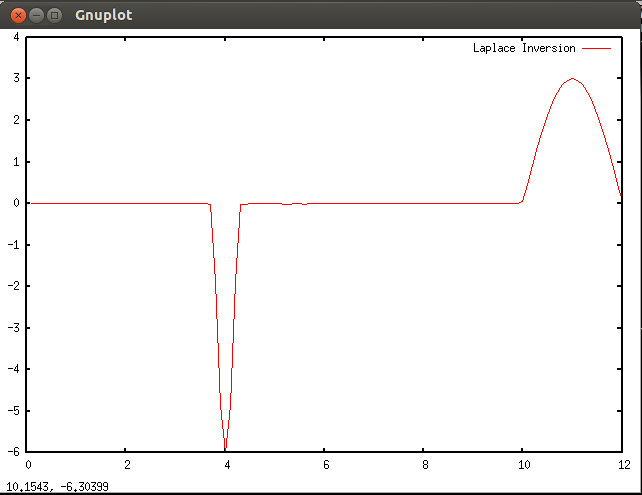
\includegraphics[width=5cm]{clock1.png}
\caption{Output of our program}
\label{clock1}
\end{figure}


But as we said before, we are French and French are all about beauty and class. The output of the program is very difficult to read, since it is very uncommon. Our spies want to act as quick as possible. We cannot conceive that they might lose some time reading time. Thus we tweak the output so that it is more readable.

\begin{figure}[!h]
\centering
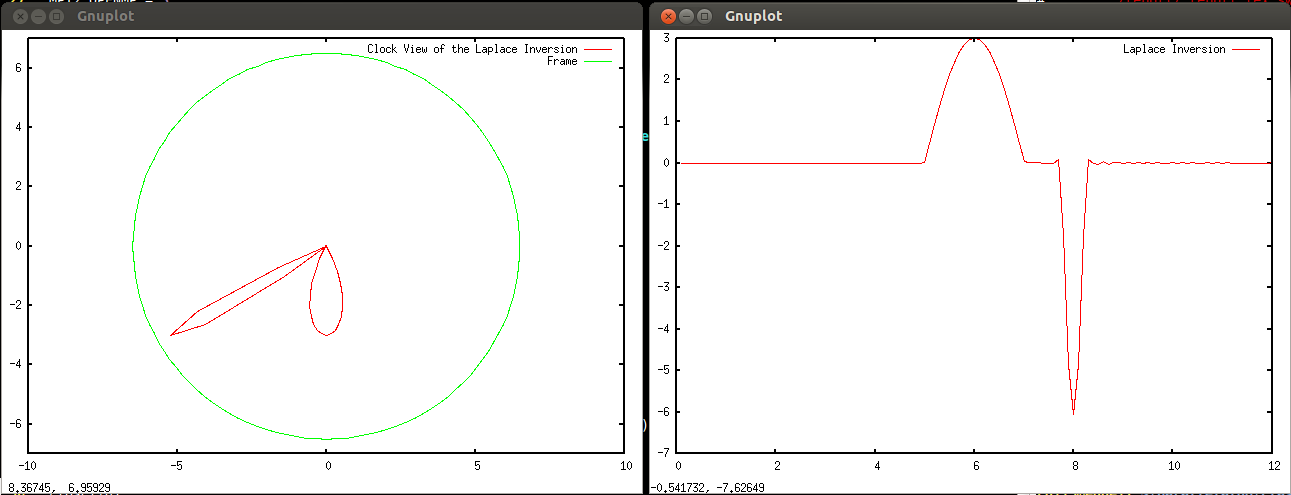
\includegraphics[width=10cm]{clock2.png}
\caption{Left the clock; Right the basic output.}
\label{clock2}
\end{figure}

This way, we are sure that our spies will have the best equipment while they are on-stage.

\begin{figure}[!h]
\centering
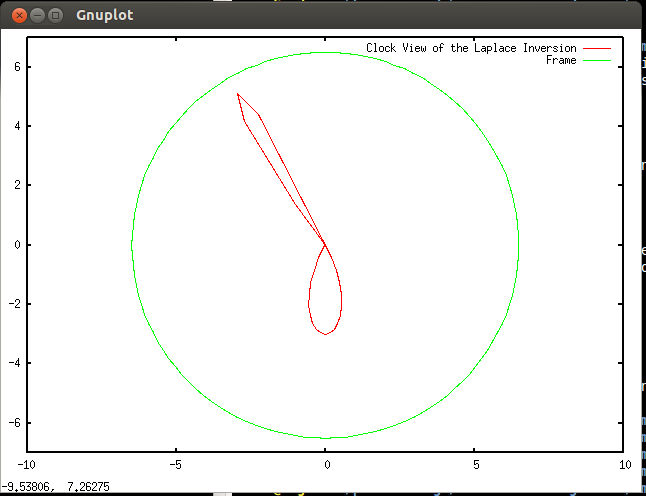
\includegraphics[width=5cm]{clock3.png}
\caption{And we cannot say we worked off the clock}
\label{clock3}
\end{figure}

\newpage

\appendix

\section{More about the program}

\subsection{Launching the program}

The main part of the project is in the repository \verb_implementation/_.

First you need to compile the programs. A complete \textit{Makefile} is provided so that you only need the command \verb_$ make_.\\

Then try \verb_$ ./whattime_ to get help about the syntax to use to launch the program.

\subsection{Overall architecture}

The general program contains 4 C++ classes:
\begin{itemize}
  \item \verb_LaplaceInv_: an abstract class that represents a Laplace transform inversion. It must be passed a function of the same signature as the mystery function \verb_L_. The virtual operator \verb_()_ called on a \verb_double_ value or a \verb_vector<double>_ is meant to return its image by the Laplace transform inversion of that function. It is supposed to be inherited multiple times for the different types of implementation of this inversion.
  \item \verb_SeqLaplaceInv_ and \verb_MPILaplaceInv_: they inherit from \verb_LaplaceInv_ and overload the operator \verb_()_. The first one implements the sequential algorithm, whereas the second one is a wrapper that calls the other executable \verb_mpicore_, which performs the computation in parallel using MPI.
  \item \verb_Plotter_: it must be passed an object of type \verb_LaplaceInv_ at construction time and provides methods that call it and then plot the output using \textit{GnuPlot}.
\end{itemize}
Its function \verb_main()_ is in \textit{start.cpp} and instanciates one of those objects depending on the parameters given by the user.

\subsection{Problems interfacing MPI with the rest of the program}
Making a global program whose executable contains MPI code would be foolish since it would use several MPI processes each time or would require to be launched with \verb_mpirun_ in every case. Hence our decision to build a different executable to handle the MPI processing, and to launch it from the global program after forking.\\

The problem then is to make those two programs communicate. We need this since the wrapper must pass arguments to its child and retrieve output data from it.\\

The first option we considered was to make the data transit by name Unix pipes. After long hours of debug, such mechanisms appeared to be very painful to program in C++ (without using system calls directly), and might have raised problems since the distributed file system NFS is used in the lab environment.\\

Thus, we decided to use a less elegant (but easier to program) solution: writing the input and output data down to normal files. The only problem with this approach is that the \verb_mpicore_ process needs a way to wake the wrapper up when it is done processing the data and has finished writing the result to the output file. In our design, such a mechanism is performed by using TCP sockets: once it has launched the \verb_mpicore_ process, the wrapper opens a server socket on the loopback interface and waits for its child to connect to it, which trigers the reading of the output file, and then the plotting.

\newpage

\begin{figure}[!h]

\includegraphics[width=7cm]{bt.jpg}
\end{figure}

\raggedleft
Nerd's and Geeks Office\\
MI6 Building\\
85 Albert Embankment\\
London SE1\\

\raggedright
\vspace{1cm}
\Huge{\textbf{Telephone Bill}}

\vspace{1cm}

\normalsize

\begin{tabularx}{\textwidth}{X X X}
  Number & Duration & Price \\
  \hline
  0700 0036 & 0h2m58s & \pounds458.92 \\
  \hline
  \textbf{Total w/o VAT} &  & \pounds458.92 \\
  \hline
  VAT 20\% & & \pounds91.78 \\
  \hline
  \textbf{Total with VAT} & & \pounds550.70 \\
\end{tabularx}


\end{document}
